\documentclass[12 pt, letterpaper]{hmcpset}
\usepackage{hw-preamble}
\usepackage{verbatim}
\usetikzlibrary{decorations.markings}

\name{Jayden Thadani}
\class{MATH 135 --- Complex Analysis}
\assignment{Homework 3}
\duedate{19th September 2024}

\begin{document}

Collaborators: Joseph Brown, Noah Leaf, Kai Mawhinney, Saheli Patel, Justin Son

\begin{problem}[1.]
	Prove that
	\[
		\int_{0}^{\infty} \sin{(x^{2})} \, dx = \int_{0}^{\infty} \cos{(x^{2})} \, dx = \frac{\sqrt{2 \pi}}{4}.
	\]
\end{problem}

\begin{solution}
	We consider the integral of $e^{-z^{2}}$ along a contour $\gamma$ — the boundary of a sector of radius $R$, centred at $0$ and with angle $\pi / 4$. Since $e^{-z^{2}}$ is entire (it is the composition of two entire functions), the integral must be zero for each $R$. Note that $\gamma$ has three smooth components. $\gamma_{1}$ is the line along the real axis from  $0$ to $R$, $\gamma_{2}$ is the arc along the circumference of a circle from $R$ to $Re^{i \pi /4}$, and $\gamma_{3}$ is the line from $R e^{i \pi /4}$ back to $0$. Thus the integrals along each of these components must sum to zero. We will consider the limit as $R \to \infty$ to evaluate the integrals in the question.

	\begin{figure}[h]\label{Figure2}
		\begin{center}
			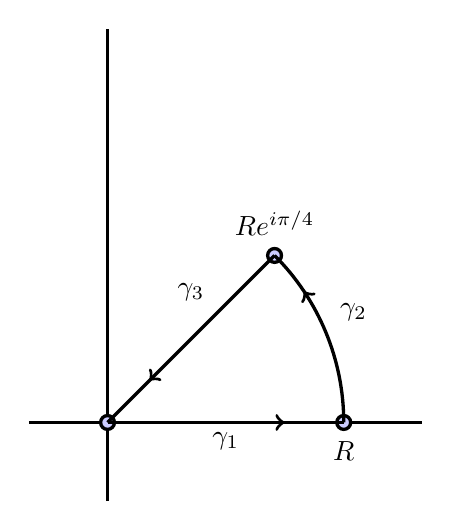
\begin{tikzpicture}[very thick, decoration={markings, mark=at position 0.75 with {\arrow{>}}},  main_node/.style={circle,fill=blue!20,draw,minimum size=0.5em,inner sep=1pt}, every loop/.style={}]
				\draw[thick](-1,0) -- node[below]{$\gamma_{1}$} ++ (5,0);
				\draw[thick](0,-1) -- (0,5);
				\node[main_node, label=below: $R$](1) at (3,0){};
				\node[main_node](2) at (0,0){};
				\node[main_node, label = above: $R e^{i \pi /4}$](3) at (2.1213,2.1213){};
				\draw[black, very thick,postaction = {decorate}](0,0) -- (3,0);
				\draw[black, very thick, postaction = {decorate}](2.1213,2.1213) -- node[above, yshift = 1 em]{$\gamma_{3}$} (0,0);
				\draw[black, very thick, postaction={decorate}] (3, 0) arc(0:45:3) node[above, midway, xshift = 1 em] {$\gamma_{2}$};
			\end{tikzpicture}
			\caption{The three smooth components of $\gamma$.}
		\end{center}
	\end{figure}

	First we will show that $\int_{\gamma_{1}} e^{-z^{2}} \, dz = \sqrt{\pi}/2$ for $R \to \infty$. Note that since $\gamma_{1}$ is just a straight line along the real axis, the integral is just
	\[
		\int_{0}^{R} e^{-x^{2}} \, dx.
	\]
	We know that
	\[
		\int_{-\infty}^{\infty} e^{-x^{2}} \, dx = \sqrt{\pi}.
	\]
	Notice that $e^{-x^{2}}$ is an even function --- $e^{-(-x)^{2}} = e^{- x^{2}}$. Thus,
	\[
		\int_{0}^{\infty} e^{-x^{2}}  \, dx = \frac{\sqrt{\pi}}{2} 
	\]
	giving us the result we want.

	Now we will show that $\int_{\gamma_{2}} e^{-z^{2}} \, dz \to 0$ as $R \to \infty$. Consider the parametrisation $z : t \mapsto R e^{i t}$	for $t \in [0, \pi / 4]$. Then
	\[
		\begin{split}
			\int_{\gamma_{2}} e^{-z^{2}} \, dz & = \int_{0}^{\pi / 4} e^{- R^{2} e^{2 i t}} \frac{dz}{dt} \, dt \\
							  & = \int_{0}^{\pi / 4} e^{- R^{2}(\cos{(2t)} - i \sin{(2t)})} iR e^{it} \, dt \\
							  & = iR \int_{0}^{\pi / 4} e^{- R^{2} \cos{(2t)}} e^{- i R^{2} \sin{(2t)}} e^{it} \, dt.
		\end{split}
	\]
	Consider the substitution $s = 2t$. Clearly $ds/2 = dt$ and $s$ ranges over $[0, \pi / 2]$. That is,
	\[
		\int_{\gamma_{2}} e^{-z^{2}} \, dz = iR \int_{0}^{\pi / 2} e^{- R^{2} \cos{s}} e^{- i R^{2} \sin{s}} e^{i s/2} \, ds.
	\]
	Notice that $e^{is/2} e^{- i R^{2} \sin{s}}$ is always on the unit circle --- we always have $\lvert e^{i s/2} e^{- i R^{2} \sin{(2t)}} \rvert = 1$. Thus,
	\[
		\begin{split}
			\left \lvert \int_{0}^{\pi / 2} e^{- R^{2} \cos{s}} e^{- i R^{2} \sin{s}} e^{i s/2} \, ds  \right \rvert & \le \left \lvert \int_{0}^{\pi/2} e^{- R^{2} \cos{s}} \lvert e^{-i R^{2} \sin{s}} e^{is/2} \rvert \, ds  \right \rvert \\
			& \le \left \lvert \int_{0}^{\pi / 2} e^{- R^{2} \cos{s}} \, ds  \right \rvert \\
			& \le \frac{\pi}{2 R^{2}}
		\end{split}
	\]
	where the last step follows by Jordan's inequality. Then clearly, as $R \to \infty$, the integral goes to $0$.

	Finally, from the integral along $\gamma_{3}$ we get expressions in the form of the integrals we want. Consider the parametrisation $z : t \to t e^{i \pi /4}$ for $t \in [0, R]$. Then
	\[
		 \begin{split}
			 \int_{\gamma_{3}} e^{-z^{2}} \, dz & = \int_{R}^{0} e^{- t^{2} e^{i \pi / 2}} \frac{dz}{dt} \, dt \\
							    & = \int_{R}^{0} e^{- i t^{2}} e^{\pi / 4} \, dt \\
							    & = e^{i \pi / 4} \int_{R}^{0} \cos{(- t^{2})} + i \sin{(- t^{2})}  \, dt \\
							    & = \frac{1 + i}{\sqrt{2}} \int_{R}^{0} \cos{(t^{2})} - i \sin{(t^{2})} \, dt \\
							    & = \frac{1}{\sqrt{2}} \left ( \int_{R}^{0} \cos{(t^{2})} \, dt + \int_{R}^{0} \sin{(t^{2})} \, dt  \right ) + \frac{i}{\sqrt{2}} \left ( \int_{R}^{0} \cos{(t^{2})} \, dt - \int_{R}^{0} \sin{(t^{2})} \, dt   \right )
		 \end{split}
	\]
	
	Consider the integrals as $R \to \infty$. Since $\int_{\gamma_{2}} e^{-z^{2}} \, dz \to 0$, we must have $\int_{\gamma_{1}} e^{-z^{2}} \, dz  = - \int_{\gamma_{3}} e^{-z^{2}} \, dz $. Substituting the evaluation of the integrals as $R \to \infty$.
	\[
		\frac{\sqrt{\pi}}{2} = \frac{1}{\sqrt{2}} \left ( \int_{0}^{\infty} \cos{(t^{2})} \, dt + \int_{0}^{\infty} \sin{(t^{2})} \, dt  \right ) + \frac{i}{\sqrt{2}} \left ( \int_{0}^{\infty} \cos{(t^{2})} \, dt - \int_{0}^{\infty} \sin{(t^{2})} \, dt   \right ).
	\]
	Since the left hand side is purely real, the right hand side must also be real. Then
	\[
		\int_{0}^{\infty} \cos{(t^{2})} \, dt = \int_{0}^{\infty} \sin{(t^{2})} \, dt.
	\]
	Thus,
	\[
		\frac{\sqrt{\pi}}{2} = \frac{2}{\sqrt{2}} \int_{0}^{\infty} \cos{(t^{2})} \, dt 
	\]
	and further,
	\[
		\int_{0}^{\infty} \sin{(x^{2})} \, dx = \int_{0}^{\infty} \cos{(x^{2})} \, dx = \frac{\sqrt{2 \pi}}{4}
	\]
	as desired.
\end{solution}

\pagebreak

\begin{problem}[2]
	Show that $\displaystyle \int_{0}^{\infty} \frac{\sin{x}}{x} \, dx = \frac{\pi}{2}$.
\end{problem}

\begin{solution}
	Consider $\gamma$ the indented semicircle with outer radius $R$ and inner radius $\varepsilon$. Since $\frac{e^{iz} - 1}{z}$, is holomorphic everywhere except at $z = 0$, it is holomorphic everywhere on $\gamma$ and in the region enclosed by it. Notice that we can break $\gamma$ into four smooth curves. $\gamma_{1}$ is a semicircle of radius $\varepsilon$, $\gamma_{2}$ is the straight line from $\varepsilon$ to $R$, $\gamma_{3}$ is a semicircle of radius $R$, and $\gamma_{4}$ is the straight line from $-R$ to $- \varepsilon$. Thus, the integrals along each of these curves must sum to zero. We will consider the limit as $R \to \infty$ and $\varepsilon \to 0$ to evaluate the integrals in the question.

	\begin{figure}[h]\label{Figure3}
		\begin{center}
			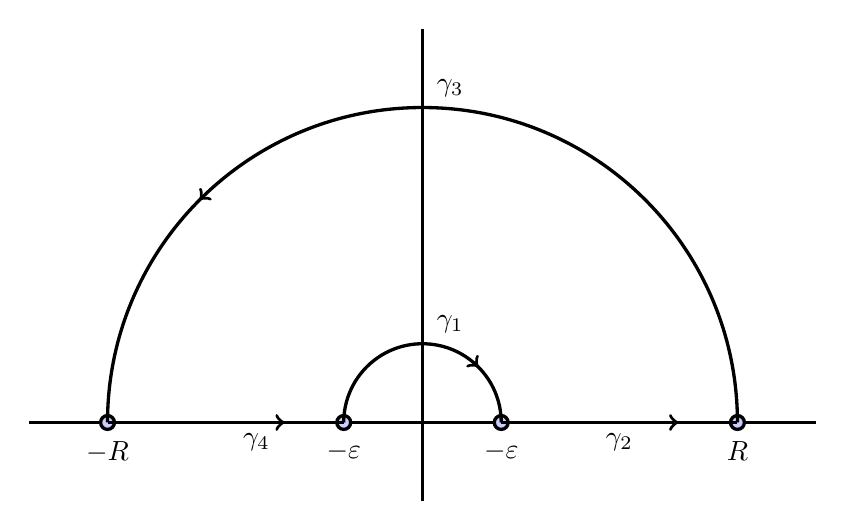
\begin{tikzpicture}[very thick, decoration={markings, mark=at position 0.75 with {\arrow{>}}},  main_node/.style={circle,fill=blue!20,draw,minimum size=0.5em,inner sep=1pt}, every loop/.style={}]
				\draw[thick](-5,0) -- (5,0);
				\draw[thick](0,-1) -- (0,5);
				\node[main_node, label=below: $R$](1) at (4,0){};
				\node[main_node, label=below: $-R$](2) at (-4,0){};
				\node[main_node, label=below: $-\varepsilon$](3) at (1,0){};
				\node[main_node, label=below: $-\varepsilon$](4) at (-1,0){};
				\draw[black, very thick,postaction = {decorate}](1,0) -- node[below, midway] {$\gamma_{2}$} (4,0);
				\draw[black, very thick, postaction = {decorate}](-4,0) node[below, midway, xshift = - 6 em] {$\gamma_{4}$} -- (-1,0);
				\draw[black, very thick, postaction = {decorate}] (4,0) arc (0:180:4) node[above, midway, xshift = 1 em]  {$\gamma_{3}$};
				\draw[black, very thick, postaction = {decorate}] (-1,0) arc (180:0:1) node[above, midway, xshift = 1 em] {$\gamma_{1}$};
			\end{tikzpicture}
			\caption{Splitting $\gamma$ into four smooth curves}
		\end{center}
	\end{figure}


	First we show that the relationship between the integrals over $\gamma_{2}$ and $\gamma_{4}$ and the integral we are trying to evaluate. Since $\gamma_{2}$ and $\gamma_{4}$ are along the real line, we can just parametrise them by functions $z : t \mapsto t$ for $t \in [\varepsilon, R]$ and $[-R, - \varepsilon]$ respectively. Thus,
	\[
		\begin{split}
			\int_{\gamma_{2}} \frac{e^{iz} - 1}{z} \, dz & = \int_{\varepsilon}^{R} \frac{e^{i t} - 1}{t} \, dt \\
								       & = \int_{\varepsilon}^{R} \frac{\cos{t} - 1}{t} \, dt + i \int_{\varepsilon}^{R} \frac{\sin{t}}{t} \, dt
		\end{split}
	\]
	and similarly,
	\[
		\int_{\gamma_{3}} \frac{e^{- i z} - 1}{z} \, dz = \int_{-R}^{- \varepsilon} \frac{\cos{t} - 1}{t} \, dt + i \int_{- R}^{- \varepsilon} \frac{\sin{t}}{t} \, dt.
	\]
	Notice that $\frac{\cos{t} - 1}{t}$ is an odd function since it is the quotient of an even function by an odd function. Also, $\frac{\sin{t}}{t}$ is an even function. Applying this fact to the sum of the integrals, we see that the integrals of $\frac{\cos{(t)} - 1}{t}$ cancel and those of $\frac{\sin{t}}{t}$ sum to give
	\[
		\begin{split}
			& \int_{\gamma_{2}} \frac{e^{- iz} - 1}{z} \, dz + \int_{\gamma_{3}} \frac{e^{-i z} - 1}{z} \, dz \\
			& = \int_{\varepsilon}^{R} \frac{\cos{t} - 1}{t} \, dt + i \int_{\varepsilon}^{R} \frac{\sin{t}}{t} \, dt + \int_{-R}^{- \varepsilon} \frac{\cos{t} - 1}{t} \, dt + i \int_{- R}^{- \varepsilon} \frac{\sin{t}}{t} \, dt \\
			& = 2i \int_{\varepsilon}^{R} \frac{\sin{t}}{t} \, dt 
		\end{split}
	\]
	Thus, as $R \to \infty$ and $\varepsilon \to 0$ we have
	\[
		\int_{\gamma_{2}} \frac{e^{-i z} - 1}{z} \, dz + \int_{\gamma_{4}} \frac{e^{-i z} - 1}{z} \, dz = 2i \int_{0}^{\infty} \frac{\sin{t}}{t} \, dt.
	\]

	Now we evaluate the integral over $\gamma_{3}$. Consider the parametrisation of $\gamma_{3}$ by $z : t \to R e^{i t}$ for $t \in [0, \pi]$. This gives us
	\[
		\begin{split}
			\int_{\gamma_{3}} \frac{e^{- i z} - 1}{z} \, dz & = \int_{0}^{\pi} \frac{e^{- i R e^{i t}}- 1}{R e^{i t}} i R e^{i t} \, dt \\
									& = i \int_{0}^{\pi} e^{- i R \cos{t}} e^{R \sin{t}} \, dt - i \int_{0}^{\pi}  \, dt \\
									& \le i \int_{0}^{\pi} \lvert e^{-i R \cos{t}} \rvert e^{R \sin{t}} \, dt - \pi i \\
									& = i \int_{0}^{\pi} e^{R \sin{t}} \, dt - \pi i 
		\end{split}
	\]
	Rewriting
	\[
		\int_{0}^{\pi} e^{R \sin{t}} \, dt = \int_{0}^{\pi /2} e^{R \sin{t}} \, dt + \int_{\pi/2}^{0} e^{- R \cos{t}} \, dt 
	\]
	it's clear to see that the integral goes to $0$ as $R \to \infty$. The first term is bounded by Jordan's inequality ---
	\[
		\int_{0}^{\pi/2} e^{R \sin{t}} \, dt \le \frac{\pi}{2 R}
	\]
	and the second term has the integrand $e^{- R \cos{t}}$ go to $0$. Thus,
	\[
		\int_{\gamma_{3}} \frac{e^{i z} - 1}{z} \, dz = - \pi i.
	\]

	Now we just need to show that the integral over $\gamma_{1}$ goes to $0$. Consider the parametrisation of $\overline{\gamma}_{1}$ ($\gamma_{1}$ oriented in the opposite direction) by $z : t \to \varepsilon e^{it}$ for $t \in [0, \pi]$. Then
	 \[
		\begin{split}
			\int_{\gamma_{1}} \frac{e^{i z} - 1}{z} \, dz & = - \int_{\overline{\gamma}_{1}} \frac{e^{iz} - 1}{z} \, dz \\
			& = - \int_{0}^{\pi} \frac{e^{\varepsilon e^{it}} - 1}{\varepsilon e^{it}} i \varepsilon e^{it} \, dt \\
			& = - i \int_{0}^{\pi} e^{\varepsilon e^{it}} - 1 \, dt.
		\end{split} 
	\]
	We claim that as $\varepsilon \to 0$, $e^{\varepsilon e^{i t}} \to 1$ uniformly (this is proven as a lemma after the problem). Then it follows that as $\varepsilon \to 0$
	\[
		-i \int_{0}^{\pi} e^{\varepsilon e^{it}} \, dt \to \int_{0}^{\pi} 1 - 1 \, dt = 0.
	\]

	Summing all the integrals, we get
	\[
		0 + 2i \int_{0}^{\infty} \frac{\sin{t}}{t} \, dt - \pi i = 0
	\]
	and thus,
	\[
		\int_{0}^{\infty} \frac{\sin{t}}{t} \, dt = \frac{\pi}{2}
	\]
	as desired.
\end{solution}

\begin{lemma}
	As $\varepsilon \to 0$, $e^{\varepsilon e^{it}}$ converges uniformly to $1$.
\end{lemma}

\begin{proof} 
	For $z = x + iy$ we know that $e^{z} = e^{x} e^{iy}$. Thus, $e^{\varepsilon e^{it}} = e^{\varepsilon \cos{t}} e^{i \varepsilon \sin{t}}$. Notice that $e^{\varepsilon \cos{t}}$ and $e^{\varepsilon e^{it}}$ converge to $1$ for $t$ in the compact set  $[0, 2 \pi]$. Thus, they converge uniformly on $[0, 2 \pi]$. Since  $\cos{t}$ and $\sin{t}$ are periodic, we have uniform convergence for all $t$. Finally, this gives us uniform convergence of the product.
\end{proof}

\pagebreak

\begin{problem}[7.]
	Suppose $f : \mathbb{D} \to \mathbb{C}$ is holomorphic. Show that the diameter $d = \sup_{z, w \in \mathbb{D}} \lvert f(z) - f(w) \rvert$ of the image of $f$ satisfies
	\[
		2 \lvert f'(0) \rvert \le d.
	\]
	Moreover, it can be shown that equality holds precisely when $f$ is linear, $f(z) = a_{0} + a_{1} z$.
\end{problem}

\begin{solution}
	As a consequence of the Cauchy integral formula we have
	\[
		2 f'(0) = \frac{1}{2 \pi i} \int_{\lvert z \rvert = r} \frac{f(z) - f(-z)}{z^{2}} \, dz
	\]
	for $r \in (0, 1)$. Note that $\lvert f(z) - f(-z) \rvert$ is bounded by the diameter of the image of $f$. That is $\lvert f(z) - f(-z) \rvert \le d$. Thus, for every circle $C$ of radius $r < 1$, we have
	\[
		\begin{split}
			2 \lvert f'(0) \rvert & = \left \lvert \frac{1}{2 \pi i} \int_{C} \frac{f(z) - f(-z)}{z^{2}} \, dz  \right \rvert \\
					      & \le \frac{1}{2 \pi} \frac{d}{r^{2}} 2 \pi r \\
					      & \le \frac{d}{r}.
		\end{split}
	\]
	Thus, we must also have
	\[
		2 \lvert f'(0) \rvert \le d.
	\]
	(If we had $2\lvert f'(0) \rvert > d$, we could choose some $r < 1$ such that $d < d / r < 2 \lvert f'(0) \rvert$).
\end{solution}

\pagebreak

\begin{problem}[9.]
	Let $\Omega$ be a bounded open subset $\mathbb{C}$, and $\varphi : \Omega \to \Omega$ be a holomorphic function. Prove that if there exists a point $z_{0} \in \Omega$ such that
	\[
		\varphi(z_{0}) = z_{0} \text{ and } \varphi'(z_{0}) = 1
	\]
	then $\varphi$ is linear.
\end{problem}

\begin{solution}
	Note that we can assume that $z_{0} = 0$. If $z_{0} \neq 0$, then $\psi(z) = \varphi(z + z_{0}) - z_{0}$ has $\psi(0) = 0$ and $\psi'(0) = \varphi'(z_{0}) (z + z_{0})' = 1$. If $\psi$ is linear, then $\psi(z) = \varphi(z + z_{0}) - z_{0}$ gives us $\psi(z) + z_{0} = \varphi(z + z_{0})$ and thus, $\psi(z + z_{0}) = \varphi(z + z_{0})$ for all $z \in \mathbb{C}$. Thus, $\varphi = \psi$ and $\varphi$ is linear too.

	Since $\varphi$ is holomorphic, we know it has a power series expansion in a disc $D$ of radius $r$ around $z_{0} = 0$. Choose $D$ such that $\overline{D} \subset \Omega$. Suppose by way of contradiction that $\varphi$ is not linear with
	\[
		\varphi(z) = z + a_{n} z^{n} + O(z^{n + 1})
	\]
	where $n$ is the first $n > 1$ such that $a_{n} \neq 0$. Let $\varphi_{k} = \underbrace{\varphi \circ \cdots \circ \varphi}_{k \text{ times}}$. Then we can see by induction that
	\[
		\varphi_{k}(z) = z + k a_{n} z^{n} + O(z^{n + 1}).
	\]
	We have the base case $k = 1$ already. Suppose $\varphi_{k}(z) = z + k a_{n} z^{n} + O(z^{n + 1})$ for some $k \in \mathbb{N}$. Then
	\[
		\begin{split}
			\varphi_{k + 1}(z) & = \varphi(\varphi_{k}(z)) \\
					   & = (z + k a_{n} z^{n} + O(z^{n + 1})) + k a_{n}(z + k a_{n} z^{n} + O(z^{n + 1}))^{n} \\
					   & = z + ka_{n}z^{n} + O(z^{n + 1}) + k a_{n} z^{n} + O(z^{n + 1}) \\
					   & = z + (k + 1) a_{n} z^{n} + O(z^{n + 1}).
		\end{split}
	\]

	Now consider the $n$th derivative of $\varphi_{k}$. We know $\varphi_{k}^{(n)}(0) = k a_{n}$, and the Cauchy inequalities give us
	\[
		\varphi_{k}^{(n)}(0) \le \frac{n! \sup_{z \in \partial D} \lvert \varphi_{k} (z) \rvert}{r^{n}}
	\]
	and thus
	\[
		a_{n} \le \frac{n! \sup_{z \in \partial D} \lvert \varphi_{k}(z) \rvert}{k r^{n}}
	\]
	But $\varphi$ is bounded on $\Omega$ since all $\varphi(z) \in \Omega$, say with $\lvert \varphi(z) \rvert < M$. Thus, $\varphi_{k}$ is also bounded by $M$ on $\Omega$. Thus
	\[
		a_{n} \le \frac{n! M}{k r^{n}}.
	\]
	Then taking the limit as $k \to \infty$, we see that $a_{n} = 0$, contradicting our assumption that $a_{n} \neq 0$. Thus, in fact there is no first $n > 1$ such that $a_{n} \neq 0$, and we have $\varphi(z) = z$ in $D$. We can then cover $\Omega$ with discs $D$ centred at a point in a previous disc (assuming connectedness of $\Omega$).
\end{solution}

\pagebreak

\begin{problem}[13.]
	Suppose $f$ is an analytic function defined everywhere in $\mathbb{C}$ and such that for each $z_{0} \in \mathbb{C}$ at least one coefficient in the expansion
	\[
		f(z) = \sum_{n = 0}^{\infty} c_{n} (z - z_{0})^{n}
	\]
	is equal to $0$. Prove that $f$ is a polynomial.
\end{problem}

\begin{solution}
	Consider some uncountable compact subset $D \subset \mathbb{C}$. Since $D$ is uncountable and we have a function from $D \to \mathbb{N}$ with $z_{0} \to n$ for where $n$ is the smallest integer with $c_{n} = 0$ in the power series expansion about $z_{0}$, there must be some $n$ such that uncountably many $z_{0} \in D$ have $c_{n} = 0$ in their power series expansion. 

	Since
	\[
		f^{(n)}(z_{0}) = \sum_{i = n}^{\infty} \frac{i!}{n!} c_{n} (z - z_{0})^{i - n},
	\]
	we must have $f^{(n)}(z_{0}) = 0$ at each of these uncountably many $z_{0}$. Since this is an infinite uncountable subset of a compact set $D$, it must have a limit point somewhere in $D$. That is, the  entire function  $f^{(n)}$ has a sequence of zeroes with a limit point in $\mathbb{C}$. Thus, $f^{(n)}$ is identically zero. Taking antiderivatives $n$ times, we recover that $f$ is a polynomial.
\end{solution}

\end{document}
